

%%%%%%%%%%%%%%%%%%%%%%%%%%%%%%%%%%%%%%%%%%%%%%%%%%%%%%%%%%%%%%%%%%%%%%%%%%%%%%%%%%%%%%%%%%%%%%%%%%%%%%%
% PACKAGES

\documentclass[a4paper, 11pt]{article}
\usepackage[utf8]{inputenc}
\usepackage[T1]{fontenc}
%\usepackage[catalan]{babel}
\usepackage{amsmath, amssymb, amsthm}
\usepackage[margin=1in]{geometry}
\usepackage{enumerate}
\usepackage{array}
\usepackage{graphicx}
\usepackage{wrapfig}
\usepackage{ragged2e}
\usepackage{subfig}
\usepackage{caption}
\usepackage{subcaption}
\usepackage[dvipsnames]{xcolor}
\usepackage{float}
\usepackage{chngcntr}
\usepackage{ragged2e}
\usepackage{multirow}
\usepackage{vmargin}
\usepackage{hyperref}
\usepackage[hidelinks]{hyperref}
\usepackage{url}
\usepackage{fancyhdr}
\usepackage{bigints}
\usepackage{listings}
\usepackage{xcolor,colortbl}


%%%%%%%%%%%%%%%%%%%%%%%%%%%%%%%%%%%%%%%%%%%%%%%%%%%%%%%%%%%%%%%%%%%%%%%%%%%%%%%%%%%%%%%%%%%%%%%%%%%%%%%
% COLORS

\definecolor{bluebell}{rgb}{0.64, 0.64, 0.82}
\definecolor{atomictangerine}{rgb}{1.0, 0.6, 0.4}
\definecolor{applegreen}{rgb}{0.55, 0.71, 0.0}
\definecolor{frenchblue}{rgb}{0.0, 0.45, 0.73}
\definecolor{darkpastelgreen}{rgb}{0.01, 0.75, 0.24}
\definecolor{darkpastelblue}{rgb}{0.47, 0.62, 0.8}
\definecolor{navy}{rgb}{0,0,128}
\definecolor{codegreen}{rgb}{0,0.6,0}
\definecolor{codegray}{rgb}{0.5,0.5,0.5}
\definecolor{codepurple}{rgb}{0.58,0,0.82}
\definecolor{backcolour}{rgb}{0.95,0.95,0.92}
\definecolor{amaranth}{rgb}{0.9, 0.17, 0.31}
\definecolor{GRAY}{rgb}{0.75, 0.75, 0.75}
\definecolor{deepfuchsia}{rgb}{0.76, 0.33, 0.76}
\definecolor{deepmagenta}{rgb}{0.8, 0.0, 0.8}
\definecolor{funcblue}{rgb}{0.36, 0.57, 0.9}
\definecolor{navy}{rgb}{0,0,128}
\definecolor{codegreen}{rgb}{0,0.6,0}
\definecolor{codegray}{rgb}{0.5,0.5,0.5}
\definecolor{codepurple}{rgb}{0.58,0,0.82}
\definecolor{backcolour}{rgb}{0.95,0.95,0.92}
\definecolor{amaranth}{rgb}{0.9, 0.17, 0.31}
\definecolor{GRAY}{rgb}{0.75, 0.75, 0.75}
\definecolor{deepfuchsia}{rgb}{0.76, 0.33, 0.76}
\definecolor{deepmagenta}{rgb}{0.8, 0.0, 0.8}
\definecolor{funcblue}{rgb}{0.36, 0.57, 0.9}

%%%%%%%%%%%%%%%%%%%%%%%%%%%%%%%%%%%%%%%%%%%%%%%%%%%%%%%%%%%%%%%%%%%%%%%%%%%%%%%%%%%%%%%%%%%%%%%%%%%%%%%
% SETTINGS

% COLOR LINK/REFERENCES
\hypersetup{colorlinks=true,
            linkcolor=blue,
            filecolor=magenta,      
            urlcolor=blue,
            }

% PAGE'S STYLE OF INITIAL PAGES
\fancypagestyle{plain}{
    \lhead[]{} % left part of the header
    \rhead[]{} % right part of the header
    \fancyfoot[]{} % borrow the foot counter page
    \lfoot[]{} % left part of the footpage
    \rfoot[]{\thepage} % right part of the footpage
    \renewcommand{\headrulewidth}{0pt} % separator line of the header
    \renewcommand{\footrulewidth}{0.5pt} % separator line of the footpage
}

% PAGE'S STYLE FOR THE THESIS
\fancypagestyle{extended_plain}{
    \lhead[]{Gerard Lahuerta Martín} % left part of the header
    \rhead[]{\leftmark} % right part of the header
    \fancyfoot[]{} % borrow the foot counter page
    \lfoot[]{} % left part of the footpage
    \rfoot[]{\thepage} % right part of the footpage
    \renewcommand{\headrulewidth}{0.5pt} % separator line of the header
    \renewcommand{\footrulewidth}{0.5pt} % separator line of the footpage
}

%%%%%%%%%%%%%%%%%%%%%%%%%%%%%%%%%%%%%%%%%%%%%%%%%%%%%%%%%%%%%%%%%%%%%%%%%%%%%%%%%%%%%%%%%%%%%%%%%%%%%%%
% CODE STYLE


%%%%%%%%%%%%%%%%%%%%%%%%%%%%%%%%%%%%%%%%%%%%%%%%%%%%%%%%%%%%%%%%%%%%%%%%%%%%%%%%%%%%%%%%%%%%%%%%%%%%%%%
% DOCUMENT

\begin{document}
\pagestyle{plain}

% TITLE
\begin{titlepage}
    \centering
    {
\includegraphics[width=0.4\textwidth]{PORTADA/UAB.png}\par}
    \vspace{1cm}
    {\bfseries\LARGE \href{https://www.uab.cat/}{Universitat Autònoma de Barcelona} \par}
    \vspace{2cm}
    {\Large Degree Thesis \par}
    \vspace{2em}
    \hline
    \vspace{1cm}
    {\scshape\Huge \textbf{Alternatives to the Steepest Gradient Descend in Neural Network training} \par}
    \vspace{1cm}
    \hline
    \vspace{2cm}
    {\Large
    \begin{figure}[h]
    \hspace{-6.5em}
        \begin{minipage}{10cm} \centering % Minipagina para la tabla. 8 cm de ancho
            \begin{tabular}{c}
                Author: \\
                \href{https://github.com/Gerard-Lahuerta}{Gerard Lahuerta Martín}
            \end{tabular}
        \end{minipage}
        \begin{minipage}{10cm} \centering % Minipagina para la tabla. 8 cm de ancho
            \begin{tabular}{c}
                Supervisor: \\
                \href{https://mat.uab.cat/~alseda/}{Dr. Lluís Alsedà Soler}
            \end{tabular}
        \end{minipage}
    \end{figure}\par}
    \vspace{2cm}
    {\scshape 
        \begin{minipage}{10cm} \centering % Minipagina para la tabla. 8 cm de ancho
            A thesis submitted in fulfilment of the requirements
            for the degree of Computational Mathematics and Data Analytics in the
        \end{minipage} 
    \par} 
    \vspace{2em}
    {\scshape\Large \href{https://www.uab.cat/ciencies}{science faculty} \par}
    \vfill
    {\Large June 2024 \par}
\end{titlepage}


\justifying
\newpage
\textcolor{white}{a}
\newpage 

% PRE SECTIONS
\addcontentsline{toc}{section}{Declaration of Authorship}
\section*{Declaration of Authorship}
\newpage
\addcontentsline{toc}{section}{Abstract}
\section*{Abstract}
\newpage
\addcontentsline{toc}{section}{Acknowledgements}
\section*{Acknowledgements}
I would like to express my gratitude to my family for their support throughout my thesis, degree, and my entire life.\\\\
I am especially grateful to my mother, Maria Montserrat, for her encouragement and guidance in facing the challenges of this thesis and my career.\\\\
I also appreciate the encouragement of my colleagues and the support of my girlfriend.\\\\
Finally, I want to give a special mention to Dr. Lluís Alsedà for guiding me through the thesis and being an inspiration.\\\\
Thank you all for everything. 
\newpage

% CONTENTS
\tableofcontents
\cleardoublepage
\addcontentsline{}{chapter}{}


\newpage
\addcontentsline{toc}{section}{Preface}
\section*{Preface}
Since in the early starts of my degree in \textit{Matemàtiques Computacionals i Analítica de Dades}, when one of my professors explains the Gradient Descend method to optimise functions, in every subject about Artificial Intelligence or Neural Networks the method used to obtain the best parameters is always the Steepest Gradient Descend.\\\\
This made me think about the nonexistence of an alternative method to optimise Neural Network's parameters, and this thought made me uncomfortable, causing me to reflect on the subject.\\\\
No professors could give me an answer to why this is the best way and why it will give the best configuration of the Neural Network's weights, they just told me that this is the fastest way to arrive to the minimum of the \textit{cost function}.\\\\
At first thought, the idea that a method whose only purpose is to minimise a value that represents how bad the model predicts seems a good proposition.\\\\
Nevertheless, there is no evidence that the results given by the method are the best ones. \\\\
I was feeling like the main idea was optimising a function without any information about it, with one algorithm that may or may not give the best result, only a relatively good one; and this way of thinking does not match with me.\\\\
This is why I am trying to change the ideology that the Steepest Gradient Descend is the best way to train Neural Network to obtain the best prediction; researching and testing different alternatives of optimization algorithms to train Neural Networks.\\\\
The final objective to this thesis is to obtain a better way to arrive to the best configuration; in other words, obtain an algorithm whose results have less error rate in Neural Network predictions (than the one obtained by Steepest Gradient Descend).


\newpage
\addcontentsline{toc}{section}{Introducción}
\section*{Introducción}
\newpage

\newpage \pagestyle{extended_plain}
\section{Neural Networks} 
Before starting programming and testing algorithms in a Neural Network is necessary to understand how Neural Networks work.\\\\
A neural Network is made of individual and independent elements connected between them, passing and managing the information through the network formed.\\\\
In this thesis we will focus on one of the simplest networks, a multilayer perceptron, to test the different methods of optimization.
\subsection{Multilayer Perceptron and Perceptron neuron}
One of the simple Neural Networks to analyse and program is the Multilayer Perceptron.\\\\
It was first proposed by Frank Rosenblat\footnote{Frank Rosenblat, psychologist and father of deep learning, check its \href{https://en.wikipedia.org/wiki/Frank_Rosenblat}{biografy}.} in 1958 (nevertheless its approach did not learn either produce accurate results).\\\\
This Neural Network is formed by elements (the artificial neurons) called \textit{Perceptrons} (which gives its name to this network). This neuron is formed by input, weight and activation functions.
\begin{figure}[h]
    \begin{minipage}{9cm}
       \begin{center}
           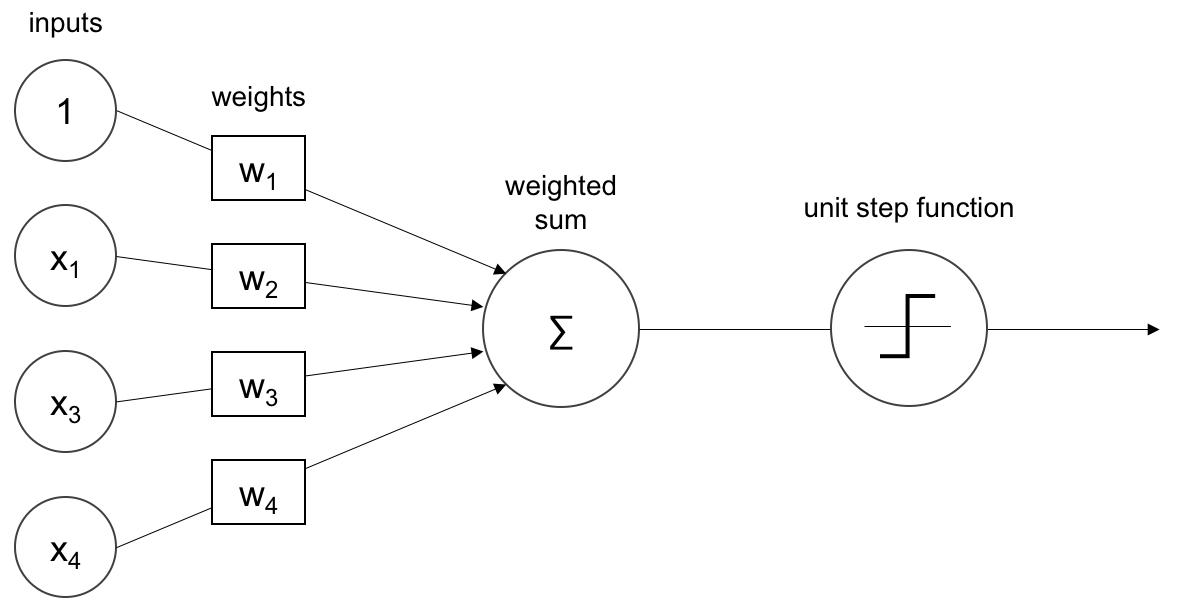
\includegraphics[width = 1 \textwidth]{Neural Network/perceptron_schema.png}
           \caption{Schema of the Perceptron neuron}
       \end{center} 
    \end{minipage}
    \hspace{1em}
    \begin{minipage}{5cm}
        The number of inputs that the Perceptron receives is variable but at least needs one input and a biaxe (represented in the picture as the input with value 1).\\\\
        All the inputs are escalated by a factor (the weights of the Perceptron) and then summed together
    \end{minipage}
\end{figure}\\
 Finally, the result of this sum is introduced in the activation function which returns the output of the neuron.\\\\
The traditional activation function used in the Multilayer Perceptron is the Sigmoid: 
$$f(x) = \frac{1}{1+e^{-w\cdot x}},\text{ where: } x,w\in\mathbb{R}^n$$
The objective of the activation function is to obtain how relevant the result of the weighted sum is.\\\\
The use of the sigmoid function as the activation function allows to represent the output of the perception as a probability (because the image of the sigmoid function is $[0,1]$).\newpage
\hspace{-1.6em}The Multilayer Perceptron is divided into layers with neurons, we can identify three types of layers:
\begin{figure}[h]
    \begin{minipage}{9cm}
        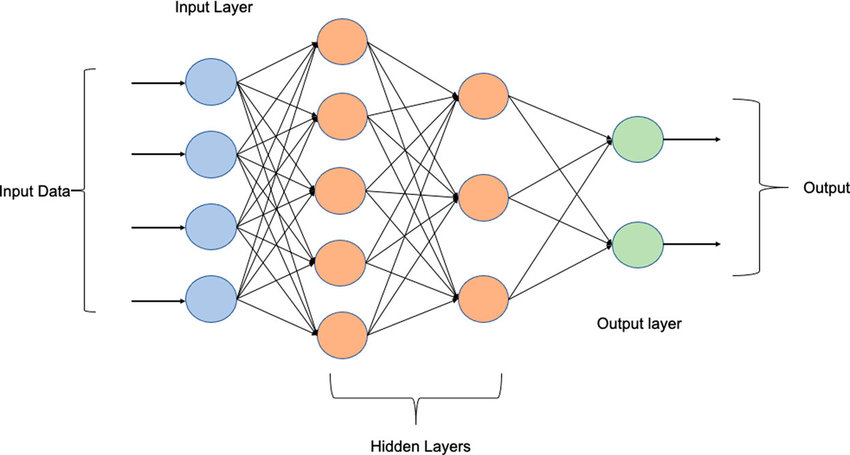
\includegraphics[width = 1 \textwidth]{Neural Network/Multi-layer-perceptron-MLP-NN-basic-Architecture.png}
           \caption{Schema of the Multilayer perceptron}
    \end{minipage}
    \hspace{1em}
    \begin{minipage}{5cm}
        \begin{itemize}
            \item \textbf{Input Layer}: The initial set of neurons of the Multilayer Perceptron.
            \item \textbf {Output Layer}: The final set of neurons of the Multilayer Perceptron.
            \item \textbf{Hidden Layers}: The set of neurons (in layers) between the input and output layers.
        \end{itemize}
    \end{minipage}
\end{figure}\\
The number of hidden layers depends on the problem and the number of neurons in each layer could not be the same.\\\\
Moreover, mention some vocabulary used in the Thesis in relation to the Neural Networks architectures:
\begin{itemize}
    \item Fully connected: Architecture with all the neurons connected between layers.
    \item Deep: Architecture where the number of layers is huge to perform complex regression or classification tasks.
\end{itemize}
Therefore, we can interpret a Multilayer Perceptron as a weighted sum of activation functions.\\\\
But, why a weighted sum of functions can perform complex tasks like classification or regression?

\subsection{Why Neural Networks works}
This topic is quite extensive, so, to simplify it, we will only consider two tasks: \textit{Classification} and \textit{Regression}.\\\\
All other capabilities (such as \textit{Natural Language Processing} or \textit{Computer Vision}) of Neural Networks can be classified in one way or another within this spectrum.\\\\
Taking this into consideration, we will now explain a simple interpretation of how Neural Networks work in these tasks.
\subsubsection{Neural Networks in Classification Tascks}
Let's imagine that we want to classify two hypothetical objects (blue and red ones) based on two relevant attributes: $A$ and $B$. If we plot these objects on a coordinate axis with attributes $A$ (x-axis) and $B$ (y-axis), one possible resulting graph could be the following one.\newpage
\begin{figure}[h]
    \begin{minipage}{8cm}
       \begin{center}
           \includegraphics[width = 1 \textwidth]{Neural Network/red_vs_blue.png}
           \caption{$AB$ attributes graph of red and blue hypothetical objects}
       \end{center} 
    \end{minipage}
    \hspace{1em}
    \begin{minipage}{6cm}
        In this scenario, one solution to classify the two objects is to divide the $AB$ attribute space (the coordinate axis) in half using the function $r(x): y = x - 1$, or in other words, by observing the sign of the expression $x - y - 1$.\\\\
        In this case, the activation function provides information about the probability of an object belonging to one of these two categories.\\\\
        If we want to classify more objects, we only need to add more 'decision functions,' as they are known. Alternatively, if the distribution of the categories is not linear, it is possible to approximate it with enough linear functions, weighted by the activation function.
    \end{minipage}
\end{figure}\\
\hspace{-1.6em}One simple example of the last situation could be if the distribution of the red and blue objects were as shown in Figure \ref{fig-example-classification}.
\begin{figure}[!h]
    \begin{minipage}{6cm}
       \begin{center}
           \includegraphics[width = 1 \textwidth]{Neural Network/red_vs_blue_case_2.png}
           \caption{Example of non-linear distribution}
           \label{fig-example-classification}
       \end{center} 
    \end{minipage}
    \hspace{1em}
    \begin{minipage}{8cm}
    In this case, we can consider dividing the space between two linear functions: $r(x): -0.62x + 0.61y = -0.38$ if $x < 2$ and $g(x): -2.14x + 0.39y = -3.72$ otherwise.\\\\
    Despite the differences between scenarios, if we want to classify a new object with this space division, the procedures are very similar to the previous one, with just a few extra steps needed.
    \begin{enumerate}
        \item Calculate the value of teach expression: $-0.62x+0.61y + 0.38$ and\\ $-2.14x+0.39y +3.72$.
        \item Evaluate each value obtained using the sigmoid activation function and take the average as the probability of belonging to one group. 
    \end{enumerate}
    \end{minipage}
\end{figure}\newpage
\hspace{-1.6em}The final function that calculates the classification (probability to belong to one group) is:
\begin{equation*}
    P(x,y) = \frac{1}{2} \left( \frac{1}{1+e^{0.38 -0.62x+0.61y}} + \frac{1}{1+e^{3.72-2.14x+0.39y}} \right)
\end{equation*} \\
This idea of the Multilayer Perceptron Neural Network have the following architecture: \\
\begin{figure}[h]
    \centering
    \includegraphics[width = 1 \textwidth]{Neural Network/diagram_example_mlp.png}
    \caption{Architecture diagram for the multilayer perception of figure \ref{fig-example-classification}}
    \label{fig:enter-label}
\end{figure}\\
In this architecture, node $N1$ could have the weights for parameters $A$ (x-axis) and $B$ (y-axis) as $\{-0.62, 0.61\}$ and a bias of $0.38$.
Node $N2$ would have weights $\{-2.14, 0.39\}$ and a bias of $3.72$.\\\\
Moreover, node $N3$ will not have a bias (its value is 0), and the weights will be ${0.5, 0.5}$.\\ 
In this case, the activation function will be the identity function.\\\\
The concept remains the same when dealing with cases involving more attributes or complex decision functions; add more layers and weights to the neural network.
\subsubsection{Neural Networks in Regression Tascks}
Let's imagine that we want to perform regression on a set of points that exhibit a certain trend, such as a polynomial trend.\\\\
In this scenario, it's important to note that any function can be approximated by an infinite sum of sigmoids:
\begin{equation}
    f(x) \approx \sum_{i = 0}^N a_i\sigma(w^T_i\cdot x + b_i)
\end{equation}
In this context, the function $f:\mathbb{R}^n \rightarrow \mathbb{R}^m$ is a continuous function to be approximated, $\sigma:\mathbb{R} \rightarrow \mathbb{R}$ is the sigmoid function, $w_i$ represents the weights of the variable $x\in\mathbb{R}^n$, $b_i$ represents the bias, and the parameter $a_i$ is a vector of size $(m,1)$ containing the weights of the sigmoid function.\\\\
This approximation is known as the \textbf{Universal Approximation Theorem}, and it enables the Multilayer Perceptron to perform both regression and classification tasks.
\subsection{Cost Function}
The most relevant application of the \textbf{Universal Approximation Theorem} in the field of Neural Networks is that it allows us to approximate cost functions, which are functions that evaluate the errors made by the model.\\
This approximation enables the model to learn by minimizing the error.\\\\
The most used cost functions are:
\begin{enumerate}
    \item \textbf{Mean Squared Error}:\\
    The Mean Squared Error (\textit{MSE}) is used in regression tasks. It estimates the error of the model. Its expression is:
    \begin{equation}
        MSE = \frac{1}{2} \sum_{i = 1}^{n} \left( \hat{y_i} - y_i \right)^2
    \end{equation}
    Where $ \hat{y}_i := f(x_i)$ represents the predicted value of the dependent variable $y_i$ to be estimated, and $n$ is the number of samples in the dataset, where $n\in\mathbb{N}$.
    \item \textbf{Cross-Entropy Loss}:\\
    The Cross-Entropy Loss (\textit{CEL}) is used in multi-class classification tasks. It estimates the accuracy of the model. Its expression is:
    \begin{equation}
        CEL = - \frac{1}{n} \sum_{i=1}^n \left(  y_{i} \cdot log(\hat{y_{i}}) \right), \text{ where } \hat{y}_i := f(x_i), n\in \mathbb{N}
    \end{equation}
     Where $ \hat{y}_i$ is the predicted probability of the \textit{i-th} data classified as the class $y_i$ and $n\in\mathbb{N}$ the number of samples.\\
\end{enumerate}
Despite the existence of these two cost functions, there are more complex functions that are widely used, such as the \textbf{Mean Absolute Error}.\\\\
This minimization process (despite the cost function) is used iteratively to determine the values of the parameters in Neural Networks, regardless of the type of task or network.\\\\
The use of iterative optimizers to obtain the best parameters for a Neural Network arises due to the complexity of finding the coefficients that minimize the cost function.\\ Moreover, in some cases, it's possible that such coefficients may not exist or cannot be obtained analytically.\\\\
This is why it's important to use differentiable cost functions in training neural networks, as they allow us to leverage the gradient of the cost function to obtain the optimal set of parameters. However, we will discuss this topic in more detail shortly.
\newpage
\subsection{BackPropagation}
The importance of using differentiable cost functions lies in their compatibility with the BackPropagation training algorithm. This algorithm relies on the derivatives of the cost function to compute the gradients for each neuron, which are then used in gradient descent optimization.\\\\
One widely used example, often employed for educational purposes to practice and understand the algorithm, is the following network:
\vspace{-1em}
\begin{figure}[h!]
    \centering
    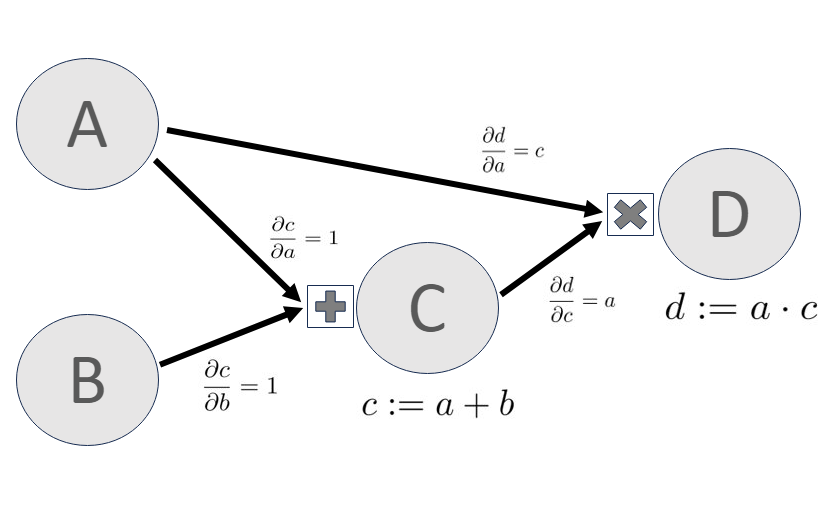
\includegraphics[width = 1 \textwidth]{Neural Network/back-graph.png}
    \vspace{-3em}
    \caption{Example of BackPropagation algorithm in simple graph}
    \label{back-prop-example}
\end{figure}\\
In the example shown in Figure \ref{back-prop-example}, if we want to modify the value of the parameter $a$ based on the output $d$, we can apply the chain rule of derivatives, as demonstrated in this case:
\begin{equation*}
    \frac{\partial D}{\partial a} = \frac{\partial d}{\partial a} + \frac{\partial d}{\partial c} \cdot \frac{\partial c}{\partial a} = c + a = 2a+b
\end{equation*}
This algorithm solves one of the biggest problems in early neural network studies related to their development and training. In practice, when a neural network is used, regardless of the task, the only information available is the input and the output.\\\\
This aspect renders the usage of neural networks with more than 2 layers (with more than 1 hidden layer) unviable.\\\\
The solution to this problem was the \textbf{Back-Propagation} algorithm, which "propagates the effects backwards", through each neuron based on its relevance to the obtained output.\\\\
This solution was first introduced by Frank Rosenblatt in 1962 for training an \textit{MLP} (Multi-Layer Perceptron). It was subsequently adopted and used in the training process of various types of neural networks due to its effectiveness, allowing the network to optimize the parameters of each neuron to minimize the error, as represented by the cost function, through \textbf{gradient descent}.
\newpage
\section{Optimizers}
\newpage\newpage
\subsection{Types of Optimizers}
\newpage\newpage
\subsection{Deterministic Optimizers}
\newpage\newpage
\subsection{Heuristic Optimizers}
\newpage\newpage
\subsection{Exploid and Explore philosofy}
\newpage 

\begin{thebibliography}{X}
\bibitem{WIKIPEDIA-MLP} \textsc{Wikipedia},
\textit{Multilayer perceptron},\\ \url{https://en.wikipedia.org/wiki/Multilayer_perceptron}
\bibitem{WIKIPEDIA-PERCERPTRON} \textsc{Wikipedia},
\textit{Perceptrón},\\ \url{https://es.wikipedia.org/wiki/Perceptr%C3%B3n}
\bibitem{WIKIPEDIA-ACTIV.FUNCT,} \textsc{Wikipedia},
\textit{Activation function},\\ \url{https://en.wikipedia.org/wiki/Activation_function}
\bibitem{WIKIPEDIA-FRANK} \textsc{Wikipedia},
\textit{Frank Rosenblatt},\\ \url{https://es.wikipedia.org/wiki/Frank_Rosenblatt}
\bibitem{WIKIPEDIA-ACTIVATINGFUNCTION} \textsc{Wikipedia},
\textit{Activating Function},\\ \url{https://en.wikipedia.org/wiki/Activating_function}
\bibitem{WIKIPEDIA-ART.NN} \textsc{Wikipedia},
\textit{Artificial neural network},\\ \url{https://en.wikipedia.org/wiki/Artificial_neural_network}
\bibitem{WIKIPEDIA-NN} \textsc{Wikipedia},
\textit{Neural network},\\ \url{https://en.wikipedia.org/wiki/Neural_network}
\bibitem{WIKIPEDIA-SIGMOID_TEOREM} \textsc{Wikipedia},
\textit{Universal Approximation Theorem},\\ \url{https://en.wikipedia.org/wiki/Universal_approximation_theorem}
\bibitem{WIKIPEDIA-MSE} \textsc{Wikipedia},
\textit{Mean Squared Error},\\ \url{https://en.wikipedia.org/wiki/Mean_squared_error}
\bibitem{WIKIPEDIA-MAE} \textsc{Wikipedia},
\textit{Mean Absolute Error},\\ \url{https://en.wikipedia.org/wiki/Mean_absolute_error}
\bibitem{WIKIPEDIA-CE} \textsc{Wikipedia},
\textit{Cross-Entropy},\\ \url{https://en.wikipedia.org/wiki/Cross-entropy}
\bibitem{WIKIPEDIA-BACKPROP} \textsc{Wikipedia},
\textit{BackPropagation},\\ \url{https://en.wikipedia.org/wiki/Backpropagation}

\bibitem{Dan} \textsc{Dantzig, G.B.} y \textsc{P. Wolfe},
<<Decomposition principle for linear programs>>,
\textit{Operations Research}, \textbf{8}, págs. 101--111, 1960.

\end{thebibliography}
\end{document}
